\section{Development view}

\textit{De development weergave illustreert het systeem van een programmeur perspectief en omvat het Software Management gedeelte.}

\begin{figure}[h]
  \centering
  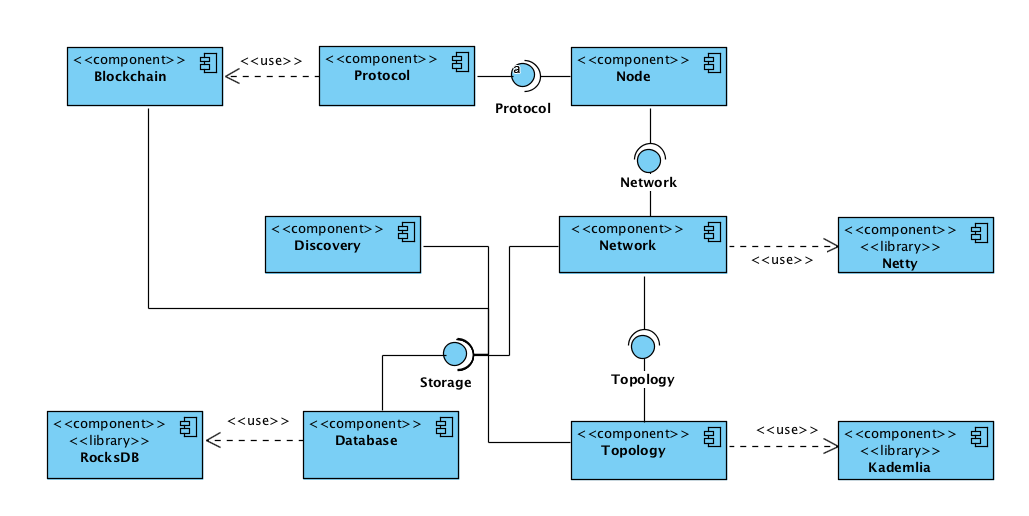
\includegraphics[width=1\textwidth]{component_diagram}
  \caption[Component Diagram] {
    Component Diagram waarin de diverse componenten en de samenwerking daartussen te zien is.
  }
  \label{diagram:component}
\end{figure}

In fig. \ref{diagram:component} is het component diagram te zien waarin de kerncomponenten van de applicatie staan. Hieronder zijn alle component individueel besproken:

\begin{itemize}
  \item \textbf{Blockchain}
  \\ Het Blockchain component bevat de logica en cryptografie om de structuur van een Blockchain op te bouwen. Een belangrijk onderdeel van het Blockchain component zijn de identiteiten die benodigd zijn voor de communicatie tussen verschillende participanten van het netwerk.
  \item \textbf{Protocol}
  \\ Het Protocol component stelt de regels op met betrekking tot het gebruik van de Blockchain data.
  \item \textbf{Node}
  \\ Het Node component bevat de functionaliteit waarmee de eindgebruiker kan interacteren.
  \item \textbf{Network}
  \\ Het Network component is een encapsulatie van de verschillende componenten die hier deel van uitmaken. Het is verantwoordelijk voor het opzetten van het gehele Peer-to-Peer netwerk.
  \item \textbf{Discovery}
  \\ Het Discovery component bevat de Peer Discovery mechanisme die gebruikt om toe te treden in het netwerk.
  \item \textbf{Topology}
  \\ Het Topology component bepaald de infrastructuur van het Peer-to-Peer netwerk.
  \item \textbf{Database}
  \\ Het Database component bevat de logica om te interacteren met de gekozen database implementatie.
\end{itemize}